\documentclass[]{article}

\usepackage[utf8]{inputenc}
\usepackage[T1]{fontenc}
%\usepackage[ngerman]{babel}
%\usepackage[babel]{csquotes}
\usepackage{tikz}
\usepackage{verbatim}
\usepackage{fancybox}
\usepackage{amsthm}
\usepackage{amsmath}
\usepackage{amssymb}
\usepackage{bm}
%\usepackage{dsfont}
%\usepackage{stmaryrd}
\usepackage{amssymb}
\usepackage{amsthm}
\usepackage{booktabs}
\usepackage{verbatim}
%\usepackage{marvosym}
\usepackage{tikz}
\usetikzlibrary{calc}
\usetikzlibrary{matrix,backgrounds}
%\usepackage[colorlinks=true, urlcolor=blue]{hyperref}
%\usepackage{graphicx}
%\usepackage{listings}
%\usepackage{algorithm2e}
 %\LinesNumbered
 %\DontPrintSemicolon
\usepackage[table,xcdraw]{}
 \usepackage[normalem]{ulem}
 \useunder{\uline}{\ul}{}

\usepackage{adjustbox}
\usepackage{algorithm}
\usepackage{algorithmicx}
\usepackage{algpseudocode}

\usepackage{longtable,booktabs}

\usepackage{struktex}
\usetikzlibrary{
  %arrows,            % Viele verschiedene Spitzen-Typen für Pfeile (mehr: http://tex.stackexchange.com/a/42679)
  automata,          % Zeichnen von Automaten
  %backgrounds,       % Hintergründe ändern
  chains,            % Abläufe darstellen
  %matrix,            % Matrizen malen
  %shadows,           % Schatten um Formen
  shapes,            % Alle zusätzlichen Formen
  %shapes.geometric,  % Mehr geometrische Formen
  %shapes.symbols,    % Mehr symbolische Formen
  %shapes.arrows,     % Mehr Pfeilformen (nicht zu verwechseln mit den Pfeilen für Pfade)
  %shapes.multipart,  % Formen unterteilen
  %shapes.callouts,   % Z.b. Sprechblasen wie man sie aus Comics kennt
  %shapes.misc,       % Diverse andere Formen, z.B. durchgestrichene Formen (crossout, strikeout)
  %spy,               % "Genaueres Hinsehen" in Diagrammen verdeutlichen
  %trees              % Bäume zeichnen
  }
\usetikzlibrary{arrows}

\tikzset{
  treenode/.style = {align=center, inner sep=0pt, text centered,
    font=\sffamily},
  tn/.style = {treenode, circle, black, font=\sffamily\bfseries, draw=black,
    fill=white, text width=1.5em},
}

\PassOptionsToPackage{unicode=true}{hyperref} % options for packages loaded elsewhere
\PassOptionsToPackage{hyphens}{url}
%
\usepackage{lmodern}
\usepackage{amssymb,amsmath}
\usepackage{ifxetex,ifluatex}
\usepackage{fixltx2e} % provides \textsubscript
\ifnum 0\ifxetex 1\fi\ifluatex 1\fi=0 % if pdftex
  \usepackage[T1]{fontenc}
  \usepackage[utf8]{inputenc}
  \usepackage{textcomp} % provides euro and other symbols
\else % if luatex or xelatex
  \usepackage{unicode-math}
  \defaultfontfeatures{Ligatures=TeX,Scale=MatchLowercase}
\fi
% use upquote if available, for straight quotes in verbatim environments
\IfFileExists{upquote.sty}{\usepackage{upquote}}{}
% use microtype if available
\IfFileExists{microtype.sty}{%
\usepackage[]{microtype}
\UseMicrotypeSet[protrusion]{basicmath} % disable protrusion for tt fonts
}{}
\IfFileExists{parskip.sty}{%
\usepackage{parskip}
}{% else
\setlength{\parindent}{0pt}
\setlength{\parskip}{6pt plus 2pt minus 1pt}
}
\usepackage{hyperref}
\hypersetup{
            pdfborder={0 0 0},
            breaklinks=true}
\urlstyle{same}  % don't use monospace font for urls
\usepackage{color}
\usepackage{fancyvrb}
\newcommand{\VerbBar}{|}
\newcommand{\VERB}{\Verb[commandchars=\\\{\}]}
\DefineVerbatimEnvironment{Highlighting}{Verbatim}{commandchars=\\\{\}}
% Add ',fontsize=\small' for more characters per line
\newenvironment{Shaded}{}{}
\newcommand{\AlertTok}[1]{\textcolor[rgb]{1.00,0.00,0.00}{\textbf{#1}}}
\newcommand{\AnnotationTok}[1]{\textcolor[rgb]{0.38,0.63,0.69}{\textbf{\textit{#1}}}}
\newcommand{\AttributeTok}[1]{\textcolor[rgb]{0.49,0.56,0.16}{#1}}
\newcommand{\BaseNTok}[1]{\textcolor[rgb]{0.25,0.63,0.44}{#1}}
\newcommand{\BuiltInTok}[1]{#1}
\newcommand{\CharTok}[1]{\textcolor[rgb]{0.25,0.44,0.63}{#1}}
\newcommand{\CommentTok}[1]{\textcolor[rgb]{0.38,0.63,0.69}{\textit{#1}}}
\newcommand{\CommentVarTok}[1]{\textcolor[rgb]{0.38,0.63,0.69}{\textbf{\textit{#1}}}}
\newcommand{\ConstantTok}[1]{\textcolor[rgb]{0.53,0.00,0.00}{#1}}
\newcommand{\ControlFlowTok}[1]{\textcolor[rgb]{0.00,0.44,0.13}{\textbf{#1}}}
\newcommand{\DataTypeTok}[1]{\textcolor[rgb]{0.56,0.13,0.00}{#1}}
\newcommand{\DecValTok}[1]{\textcolor[rgb]{0.25,0.63,0.44}{#1}}
\newcommand{\DocumentationTok}[1]{\textcolor[rgb]{0.73,0.13,0.13}{\textit{#1}}}
\newcommand{\ErrorTok}[1]{\textcolor[rgb]{1.00,0.00,0.00}{\textbf{#1}}}
\newcommand{\ExtensionTok}[1]{#1}
\newcommand{\FloatTok}[1]{\textcolor[rgb]{0.25,0.63,0.44}{#1}}
\newcommand{\FunctionTok}[1]{\textcolor[rgb]{0.02,0.16,0.49}{#1}}
\newcommand{\ImportTok}[1]{#1}
\newcommand{\InformationTok}[1]{\textcolor[rgb]{0.38,0.63,0.69}{\textbf{\textit{#1}}}}
\newcommand{\KeywordTok}[1]{\textcolor[rgb]{0.00,0.44,0.13}{\textbf{#1}}}
\newcommand{\NormalTok}[1]{#1}
\newcommand{\OperatorTok}[1]{\textcolor[rgb]{0.40,0.40,0.40}{#1}}
\newcommand{\OtherTok}[1]{\textcolor[rgb]{0.00,0.44,0.13}{#1}}
\newcommand{\PreprocessorTok}[1]{\textcolor[rgb]{0.74,0.48,0.00}{#1}}
\newcommand{\RegionMarkerTok}[1]{#1}
\newcommand{\SpecialCharTok}[1]{\textcolor[rgb]{0.25,0.44,0.63}{#1}}
\newcommand{\SpecialStringTok}[1]{\textcolor[rgb]{0.73,0.40,0.53}{#1}}
\newcommand{\StringTok}[1]{\textcolor[rgb]{0.25,0.44,0.63}{#1}}
\newcommand{\VariableTok}[1]{\textcolor[rgb]{0.10,0.09,0.49}{#1}}
\newcommand{\VerbatimStringTok}[1]{\textcolor[rgb]{0.25,0.44,0.63}{#1}}
\newcommand{\WarningTok}[1]{\textcolor[rgb]{0.38,0.63,0.69}{\textbf{\textit{#1}}}}
\setlength{\emergencystretch}{3em}  % prevent overfull lines
\providecommand{\tightlist}{%
  \setlength{\itemsep}{0pt}\setlength{\parskip}{0pt}}
\setcounter{secnumdepth}{0}
% Redefines (sub)paragraphs to behave more like sections
\ifx\paragraph\undefined\else
\let\oldparagraph\paragraph
\renewcommand{\paragraph}[1]{\oldparagraph{#1}\mbox{}}
\fi
\ifx\subparagraph\undefined\else
\let\oldsubparagraph\subparagraph
\renewcommand{\subparagraph}[1]{\oldsubparagraph{#1}\mbox{}}
\fi

% set default figure placement to htbp
\makeatletter
\def\fps@figure{htbp}
\makeatother

\date{}

\begin{document}

{\footnotesize \parindent0em
    {\sc Universität Konstanz} \hfill {\sc Software Projekt, Gruppe 2.1}\par
    {\sc Fachbereich Informatik \& Informationswissenschaft} \hfill Sommersemester 19 \par
    David Boetius \hfill \today\par
    \bigskip
    \begin{center}
    {\LARGE\bf Milestone 2 StressMinimization Benchmark}
    \bigskip
    \end{center}
}

\section{Einführung}

In den benchmarks wurde einzig die Ausführungszeit in Millisekunden gemessen (Median der Ausführungszeit bei in der Regel 20 Runden Warmup und 50 Runden für den Benchmark, für die Benchmarks mit mehr als 1000 Knoten wurde hiervon abgewichen). \\ 
Der reservierte Arbeitsspeicher in der VM nach der Ausführung der warmup Runden wurde auch gemessen, gibt aber nicht wieder wie hoch der Speicherbedarf für die eigentliche Ausführung des Algorithmus wirklich war. Der in VANTED angezeigte verwendete Arbeitspeicher während der Ausführung war typischerweise etwa halb so groß, wie der von der VM als total available memory angegebene Arbeitsspeicher. \\
Alle Messungen wurden auf einem iMac Ende 2013, Intel i5, 4 Kerne, 16 GB Arbeitsspeicher ausgeführt. \\
Gebenchmarks wurden Sternen Graphen, Rad Graphen (Sternen Graphen, bei denen die äußeren Knoten zusätzlich zu einem Kreis verbunden wurden), vollständige Graphen, Pfade, sowie Barabais Albert Netzwerke, Watts Strogatz Netzwerke und Sierpinsky Dreiecke. \\
Barabais Albert Netzwerke und Watts Strogatz Netzwerke wurden gewählt um Graphen zu benchmarken, die eine gewisse Ähnlichkeit zu bestimmten nicht künstlich erzeugten Graphen haben. 

\section{Asymptotische Performance}

Abbildung~\ref{fig:watts-strogatz-barabasi-albert-runtime} zeigt die Laufzeiten für Watts-Strogatz und Barabasi-Albert Netzwerke mit Knotenanzahlen zwischen $100$ und $1000$ an. \\
Es zeichnet sich die quadratische Laufzeitklasse der Berechnung ab.
 Abbildung~\ref{fig:watts-strogatz-barabasi-albert-edges} zeigt für diese Graphen die respektiven Kantenanzahlen. Mit dieser zusätzlichen Information können wir in der ersten Abbildung den Unterschied zwischen den beiden Netzwerken erklären. Hier spielt die Berechnung der Distanzen ein, die von der Anzahl der Kanten abhängt. \\
 In den Abbildungen kommen für einzelne Knotenzahlen mehrere Laufzeiten vor, weil für diese in verschiedenen Benchmark-Suits Messwerte vorlagen. 

\begin{figure}
    \centering
	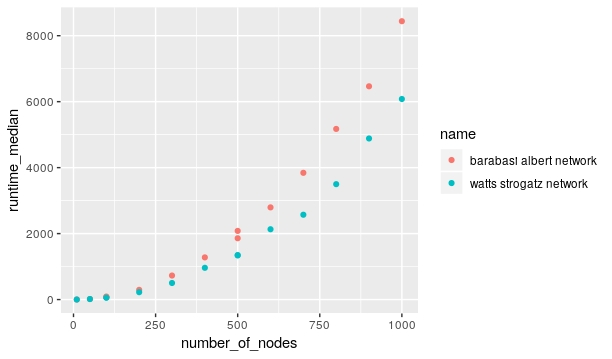
\includegraphics[width=1\textwidth]{watts-strogatz-barabasi-albert-comparison-runtime.jpeg}
    \caption{Laufzeiten der Ausführung des Stress Minimization Prozesses auf Watts-Strogatz und Barabasi-Albert Netzwerken für $n \in [100, 1000]$}
    \label{fig:watts-strogatz-barabasi-albert-runtime}
\end{figure}

\begin{figure}
    \centering
	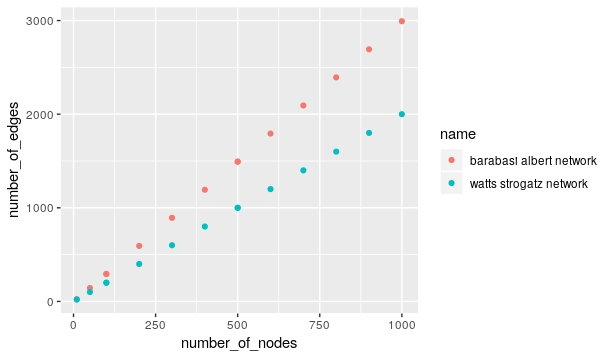
\includegraphics[width=1\textwidth]{watts-strogatz-barabasi-albert-comparison-nodes-to-edges.jpeg}
    \caption{Kantenanzahlen von Watts-Strogatz und Barabasi-Albert Netzwerken}
    \label{fig:watts-strogatz-barabasi-albert-edges}
\end{figure}

\section{Performance für verschiedene Typen von Graphen}

In den Abbildungen~\ref{fig:graphs-nodes}~und~\ref{fig:graphs-edges} sehen wir die Laufzeiten des Stress Minimization Algorithmus für verschiedene Typen von Graphen: Stern Graphen, Rad Graphen, vollständige Graphen, Pfade und wiederum Watts-Strogatz und Barabasi-Albert Natzwerken. \\
Für Pfade lag die Ausführungszeit immer wesentlich höher als bei den anderen Graphen, so dass kein Benchmark mehr mit $n = 500$ ausgeführt wurde. Die Ausführungszeit des Algorithmus hängt gegenwärtig also auch wesentlich von anderen Faktoren als nur der Knotenzahl und der Kantenzahl ab. Für diese Graphen führt der Algorithmus sehr viele Iterationen aus, wobei das berechnete Layout einen sehr geringen Stress ($\approx 0$) aufweißt. Durch den geringen Stress erfüllen die Veränderungen des Stress in den Itterationsschritten immernoch das Kriterium $\frac{stress_{prev} - stress_{new}}{stress_{prev}} > 1 \cdot 10^{-4}$ aber die absolute Änderung im Stress ist gering. \\
Ansonsten können wir wiederum sehen, dass auch die Kantenanzahl signifikanten Einfluss auf die Ausführungszeit haben kann (vollständiger Graph mit $n = 500$) und wir können die tatsächlichen Ausführungszeiten abschätzen. 

\begin{figure}
    \centering
	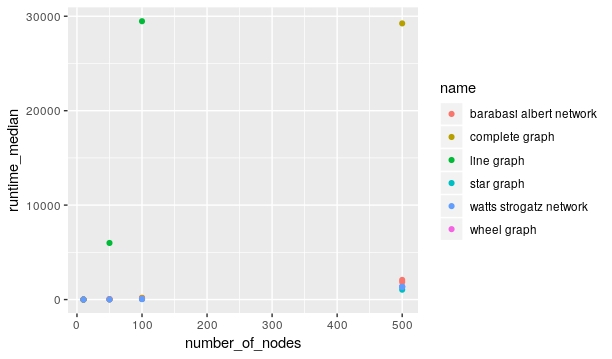
\includegraphics[width=1\textwidth]{standard_benchmarks_nodes.jpeg}
    \caption{Laufzeiten für verschiedene Graphtypen nach Knotenzahl}
    \label{fig:graphs-nodes}
\end{figure}

\begin{figure}
    \centering
	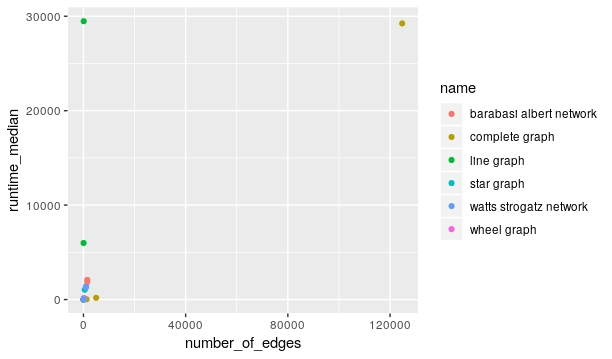
\includegraphics[width=1\textwidth]{standard_benchmarks_edges.jpeg}
    \caption{Laufzeiten für verschiedene Graphtypen nach Kantenzahl}
    \label{fig:graphs-edges}
\end{figure}

\section{Sierpisky Dreiecke: Faktoren und Speicherprobleme}

Abbildung~\ref{fig:sierpisky} zeigt Laufzeiten für Sierpinsky Dreiecke mit Rekursionstiefen zwischen 3 und 8 an. \\
Hieraus können wir beispielhaft ablesen, in welchen Bereichen die Laufzeiten für Graphen mit mehr als $1000$ Knoten liegen. \\
Während die Auführungszeit für ein Sierpinsky Dreieck mit etwa $1000$ Knoten circa bei 20 Sekunden lag, stieg dieser Wert für die weiteren Rekursionstiefen auf etwa 4 Minuten ($n \approx 3000$), bzw. 50 Minuten ($n \approx 10000$) an. \\

Für das Sierpinsky Dreieck mit Rekursionstiefe 9 ($n = 29526$) stürzte das Programm ab, weil der Heap-Speicherplatz (ca. 4 GB) nicht ausreichte. Hier wurde die maximale Größe des Heap erreicht, der für die VM eingestellt war. \\

\begin{figure}
    \centering
	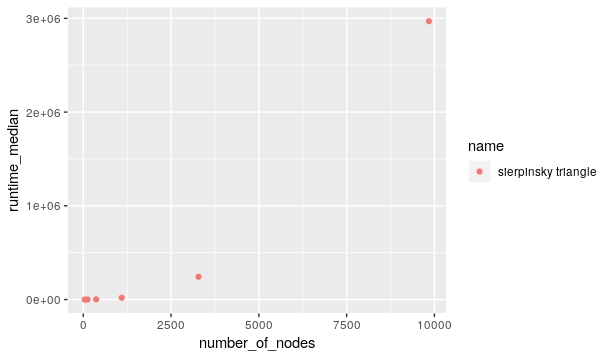
\includegraphics[width=1\textwidth]{sierpinsky.jpeg}
    \caption{Laufzeiten für Sierpinsky Dreiecke bis zur Tiefe 8}
    \label{fig:sierpisky}
\end{figure}

\end{document}